\documentclass[11pt, oneside]{article}   	% use "amsart" instead of "article" for AMSLaTeX format
\usepackage{geometry}                		% See geometry.pdf to learn the layout options. There are lots.
\geometry{letterpaper}                   		% ... or a4paper or a5paper or ... 
%\geometry{landscape}                		% Activate for rotated page geometry
%\usepackage[parfill]{parskip}    		% Activate to begin paragraphs with an empty line rather than an indent
\usepackage{graphicx}				% Use pdf, png, jpg, or eps§ with pdflatex; use eps in DVI mode
\usepackage{amsmath}								% TeX will automatically convert eps --> pdf in pdflatex		
\usepackage{amssymb}
\usepackage[final]{pdfpages}
\usepackage{listings}
\usepackage{color}

\definecolor{dkgreen}{rgb}{0,0.6,0}
\definecolor{gray}{rgb}{0.5,0.5,0.5}
\definecolor{mauve}{rgb}{0.58,0,0.82}

\lstset{language=Matlab,%
    %basicstyle=\color{red},
    breaklines=true,%
    morekeywords={matlab2tikz},
    keywordstyle=\color{blue},%
    morekeywords=[2]{1}, keywordstyle=[2]{\color{black}},
    identifierstyle=\color{black},%
    stringstyle=\color{mauve},
    commentstyle=\color{dkgreen},%
    showstringspaces=false,%without this there will be a symbol in the places where there is a space
    numbers=left,%
    numberstyle={\tiny \color{black}},% size of the numbers
    numbersep=9pt, % this defines how far the numbers are from the text
    emph=[1]{for,end,break},emphstyle=[1]\color{red}, %some words to emphasise
    %emph=[2]{word1,word2}, emphstyle=[2]{style},    
}





\title{Millikan's Oil Drop Experiment}
\author{David Abramov}	

\begin{document}
\maketitle

\section{Abstract}
	
\section{Introduction}
	Robert Andrews Millikan (1868-1953) is credited with his achievement unveiling with accuracy and precision the quantized nature of charged particles through developing and improving upon preexisting apparatus designs (Franklin, p. 1). Earlier experiments, such as J.J. Thompson's cathode ray in 1897, determined that negatively charged particles existed, however, he was only able to find a mass-to-charge (m/e) ratio of these negatively charged particles. In order to determine that mass of one of these negatively charged particles, first a method had to be developed to measure individual charges.
	
	Early experiments to quantify e did not provide evidence for a single unit of charge, as the movement of clouds of charged water droplets in the presence and absence of an electric field was initially measured. Instead of measuring the charge of individual droplets, this technique measured the charge of the entire cloud. Measurements of charge using this method were unreliable, as the clouds would quickly evaporate, and there was no measurement of the charge of a single droplet. 
	
	Millikan improved upon this experimental design namely through the substitution of oil for water, which greatly reduced the effects of evaporation. He also managed to tune the electric field of his apparatus such that the droplets could be suspended in midair, effectively counterbalancing the force of gravity. By measuring the time required for an oil drop to move the same distance upward and downward (in the presence and absence of an electric field, respectively), Millikan was able to calculate the mass of an oil drop and its charge.
\section{Experimental Method and Apparatus}

	A PASCO Scientific AP-8210 Millikan Oil Drop Apparatus was used (Fig. 1). The light source was replaced with an LED flashlight mounted to a bar stand. The apparatus was set up and calibrated following the procedures listed in the instruction manual. I recorded the rise and fall time of six different oil drops over one major grid space (0.5 mm), as recommended by the PASCO instruction manual, taking into account time to reach terminal velocity.

\includegraphics{fig1}
Figure 1. PASCO Scientific 8210 Millikan Oil Drop Apparatus. The included light source was replaced with an LED flashlight mounted to a bar stand.
\section{Data Analysis and Results}
	The PASCO instruction manual listed a derivation of the Stokes' Law equation that allowed me to calculate the mass of the oil drop, and subsequently, the amount of charge on one drop. 

The forces acting on a falling oil drop in the absence of an electric field can be described using the equation

\begin{equation}
mg=kv_{f}
\end{equation}

\noindent where $m$ is the mass of the drop, $g$ is the acceleration due to gravity (9.80665 m/s$^2$),  $k$ is the coefficient of friction between the oil drop and air, and $v_{f}$ is the fall velocity (which points up because drag operates as a frictional force in the direction opposite to the motion). The forces acting on an oil drop that is rising can be described by the following equation,

\begin{equation}
Eq=mg+kv_{r}
\end{equation}

\noindent where $E$ is the electric field, $q$ is the charge of the oil drop, and $v_{r}$ is the velocity of rise (which points down because drag operates in the direction opposite of motion). These equations can be combined by solving for $k$ in each case, setting the resultant equations equal to each other, subsequently eliminating $k$.

\begin{equation}
q=\frac{mg(v_{f}+v_{r})}{Ev_{f}}
\end{equation}

The mass of the oil drop can be rewritten using the volume of a sphere, where the radius $a$ can be calculated using Stokes' Law, which relates the radius of a spherical object to the viscosity of the medium it is falling through ($\eta$) to its velocity and density ($\rho$=800 kg/m$^3$). However, Stokes' law becomes less accurate as the velocity falls below 0.1 cm/s (10-100 times greater than the measured velocities in this experiment), so a viscosity correction factor was used in the derivation.

\begin{equation}
m=\frac{4}{3}\pi a^3\rho=\frac{4}{3}\pi\Bigg[\sqrt{(\frac{b}{2p})^2+\frac{9\eta v_{f}}{2g\rho}-\frac{b}{2p}}^3\Bigg]\rho
\end{equation}

\noindent Plugging in this equation for mass into the charge equation results in following equation.

\begin{equation}
q=\frac{4}{3}\pi\rho g\Bigg[\sqrt{(\frac{b}{2p})^2+\frac{9\eta v_{f}}{2g\rho}-\frac{b}{2p}}^3\Bigg]\frac{(v_{f}+v_{r})}{Ev_{f}}
\end{equation}

\noindent The electric field $E$ can be rewritten using the following conversion equation,

\begin{equation}
E(e.s.u.)=\frac{V(volts)}{300d(cm)}
\end{equation}

\noindent where $d$ is the distance between the plates in the condenser (0.0076 cm). This can be plugged in for $E$, giving a final equation for $q$ as the following,

\begin{equation}
q=\frac{4}{3}\pi\rho g\Bigg[\sqrt{(\frac{b}{2p})^2+\frac{9\eta v_{f}}{2g\rho}-\frac{b}{2p}}^3\Bigg]\frac{(v_{f}+v_{r})300d}{Vv_{f}}
\end{equation}

\noindent where $q$ is the charge of the droplet (C), $d$ is the separation of the plates in the condenser (m), $\rho$ is the density of oil (approximately 800 kg/m$^3$), $g$ is the acceleration of gravity (9.80665 m/s$^2$), $\eta$ is the viscosity of air in poise (Ns/m$^2$), $b$ is a constant (8.20 x 10$^-$$^3$ Pa$\cdot$m), $p$ is barometric pressure (Pa), $a$ is the radius of the droplet (m), $v_{f}$ is the velocity of fall (m/s), $v_{r}$ is the velocity of rise (m/s), and $V$ is the potential difference across the plates (V).

I found the viscosity of air, $\eta$, by measuring the thermistor resistance to find the temperature of the chamber (Appendix B of the PASCO Manual) and comparing that value to the viscosity of dry air as a function of temperature as shown in Appendix A of the PASCO apparatus manual.

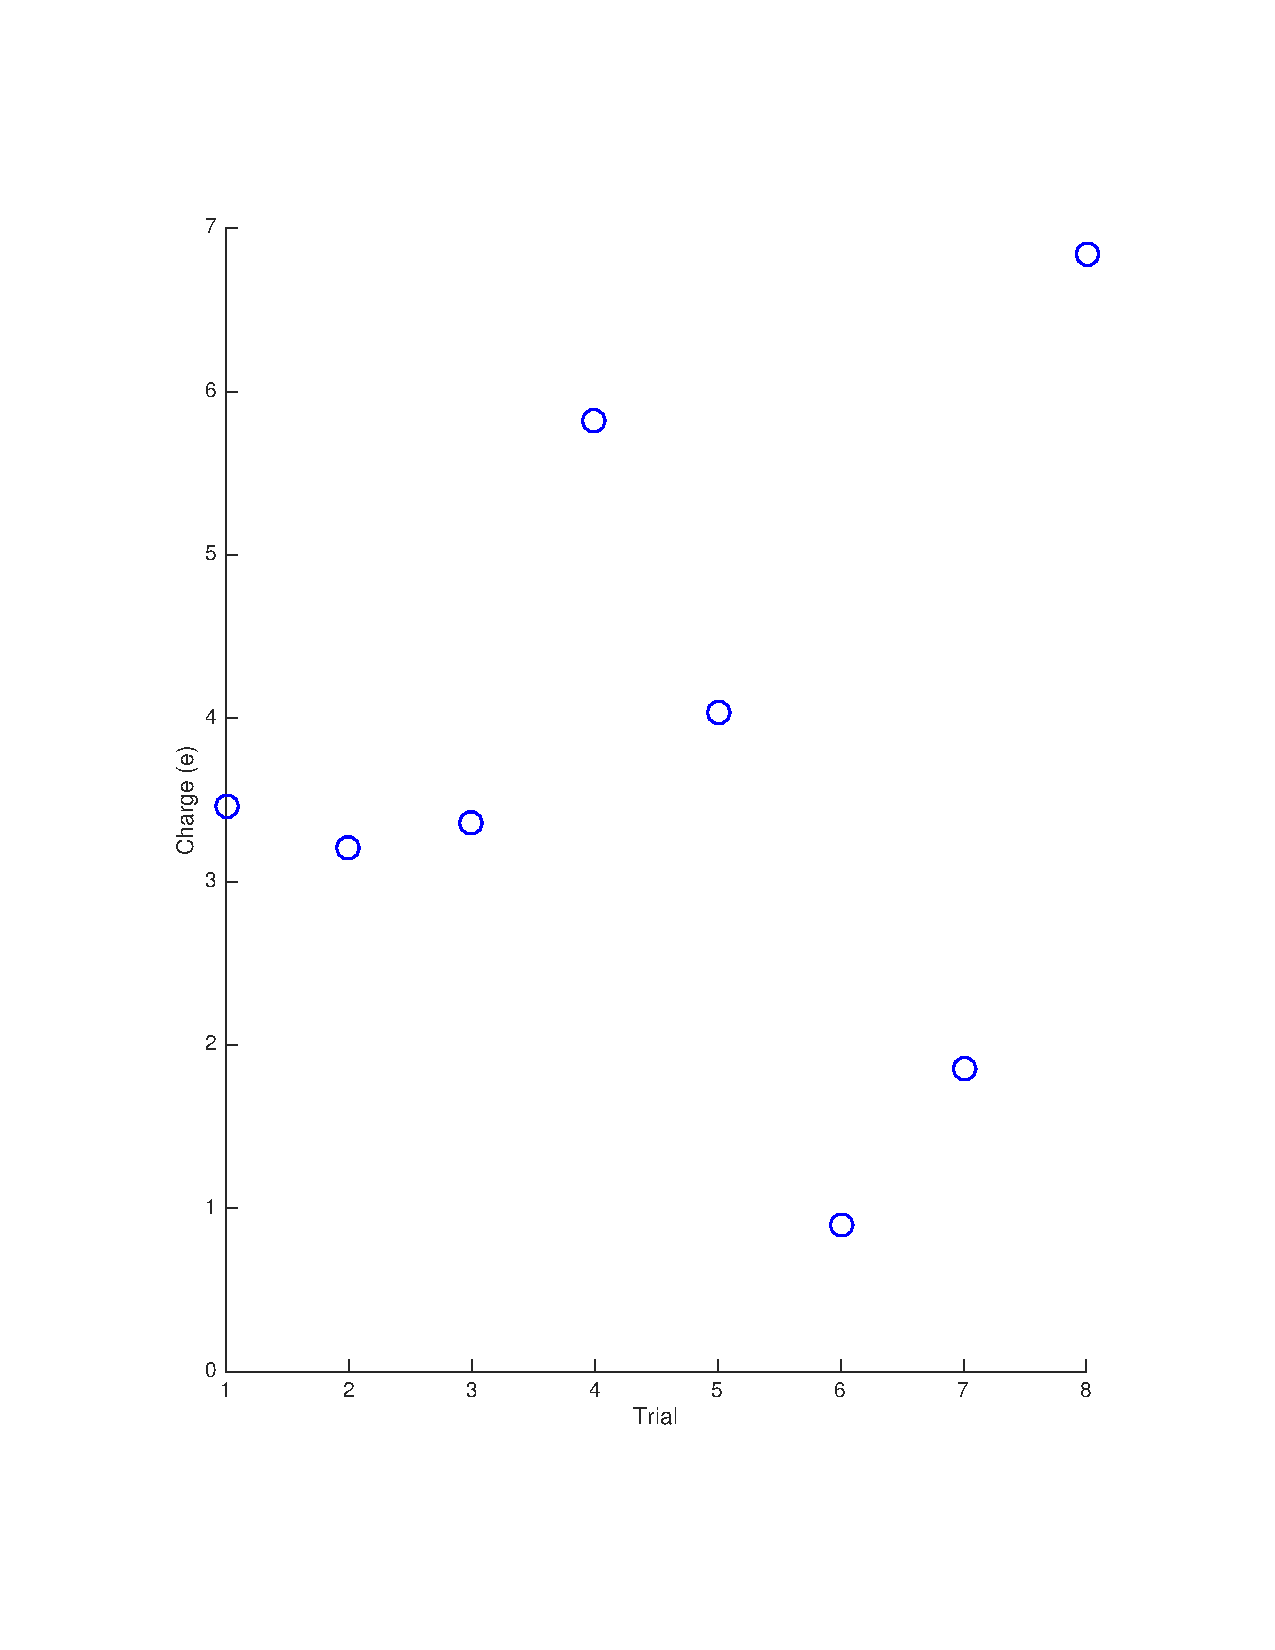
\includepdf[pages=-]{fig2.pdf}
Figure 2. Oil droplet charge measured using Millikan's Oil Drop Apparatus. Trials 5 and 6 were measurements of the same droplet before and after a spontaneous drop in charge. Likewise, trials 7 and 8 were of the same droplet, although there was an increase in charge after ionization.
\section{Calibration, Errors, and Measurement Precision}

\section{Conclusions}

\section{Discussion}

%How does the scientific community reach consensus on a theory or experiment (e.g. the charge of an electron)? How does this compare and contrast with the way a Wikipedia page reaches consensus?

%Does Chauvenet's criterion apply to Millikan's oil drop data as described in the readings above? Is it applicable, and if so, would it have changed his results?

%Does Chauvenet's criterion apply to my oil drop data? Is it applicable, and if so, would it have changed my results?

\section{References}

Taylor's Error Analysis, Ch. 1-6

Junior Year Experiential Learning Description (D2L)

Cargo Cult Science by Richard Feynman (D2L)

A. Franklin, "Millikan's Oil-Drop Experiments," The Chemical Educator 2, 1 (1997)
Sections 10-13 of R.A. Millikan, "On the Elementary Electrical Charge and the Avogadro Constant," Phys. Rec. 2, 109-143 (1913).

G. LaRue et. al., "Observation of Fractional Charge of (1/3)e on Matter," Phys. Rev. Lett. 46, 967-970 (1981).
Sections I and V of I. T. Lee et al., "Large bulk matter search for fractional charge particles," Phys. Rev. D 66, 012002 (2002).

http://www.openwetware.org/images/8/8b/Ap8210.jpg

\section{Appendix}

Appendix A: Oil Drop Charge Plotter. This script (q.m) written in MatLAB loads oil drop data saved in a .mat container. This data was imported from an Excel spreadsheet containing the raw data in the included folder labeled "data." The script then calls the function (oildrop.m) (Appendix B) to calculate the charge of each oil drop.

\begin{lstlisting}
load('data.mat');
a = size(bf);
charge = zeros(a);
for c = 1:a
    charge(c) = oil_drop(br(c),bf(c),V(c),P(c),n(c));
end

cc = charge/1.6e-19;
sc = sort(cc);
hold on
plot(cc, 'bo', 'MarkerSize', 11)
%plot(sc, 'o', 'MarkerSize', 12)
xlabel('Trial','FontSize',15);
ylabel('Charge (e)','FontSize',15);
\end{lstlisting}

Appendix B: Calculation of Oil Drop Charge. This function $oildrop.m$ written in MatLAB takes the average rise time $br$, average fall time $bf$, the voltage provided by the power supply $V$, the room air pressure $P$ (measured using the Android App called Sensor Sense on my Samsun Galaxy S4 cell phone), and the viscosity of air $n$, which was calculated by measuring the thermistor resistance to find the temperature of the chamber (Appendix B of the PASCO Manual) and comparing that value to the viscosity of dry air as a function of temperature as shown in Appendix A of the PASCO apparatus manual.

\begin{lstlisting}
function [ q ] = oildrop(br,bf,V,P,n)

ro = 800; %density of oil in kg/m^3 (~0.8 g/cm^3)
g = 9.80665; %m/s^2
b = 8.2e-3; % constant in Pa*m
p = P*100; %barometric pressure in Pa
%omega = 2.15; % Mohm
n = n; %viscosity of air in poise Ns/m^2
vf = bf/1000; %velocity of fall in m/s
vr = br/1000; %velocity of rise in m/s
V = V; %potential difference across the plates in Volts
d = 0.0076; %width of plastic spacer
E = V/(300*d);

q = (4/3)*pi*ro*g*((sqrt((b/(2*p))^2+((9*n*vf)/(2*g*ro)))-(b/(2*p)))^3)*((vf+vr)/(E*vf));

end
\end{lstlisting}





\end{document}